
\documentclass[a4paper,UKenglish,cleveref, autoref, thm-restate]{lipics-v2021}

\usepackage{amsmath,amssymb,amsthm}
\usepackage{stmaryrd}
\usepackage{proof}
\usepackage{tikz}
	\usetikzlibrary{calc}

\usepackage{FMC}


\bibliographystyle{plainurl}


% - - - - - - - - - - - - - - -


%\newcommand\looppicx[1]{
%\begin{tikzpicture}[thick,x=12pt,y=12pt,outer sep=0pt,inner sep=2pt]
%	\coordinate (m) at (0,0);
%	
%	\begin{scope}[->,>=stealth,anchor=north]
%		\ifx#11
%		\draw (m)--node[pos=0.6,anchor=east]{$\termcolor\scriptstyle{i\vphantom j\,}$} (-1,-2) node {$\vphantom:\typecolor\scriptstyle{p}$};
%		\draw (m)--node[pos=0.6,anchor=west]{\,$\termcolor\scriptstyle{j}$}            ( 1,-2) node {$\vphantom:\typecolor\scriptstyle{q}$};
%		\else
%		\draw (m)--node[pos=0.6,anchor=east]{$\termcolor\scriptstyle{i\vphantom j\,}$} (-1,-2) node {$\vphantom:\typecolor\scriptstyle{\frac p{1-q}}$};
%		\fi
%	\end{scope}
%	
%	\node (x) at (0,-3) {};
%	
%	\coordinate (a) at ( .85,-1.7);% \node[gray,circle,draw,inner sep=0pt,minimum size=2pt] at (a) {};
%	\coordinate (b) at (1.25,-1.6);% \node[gray,circle,draw,inner sep=0pt,minimum size=2pt] at (b) {};
%	
%    	\ifx#10
%		%\draw (m) [rounded corners=20pt] -- (1.25,-2.5) [rounded corners=5pt] -- (1.25,1.5) -- (0,1.5) -- (0,1);
%		\draw[rounded corners=5pt] (m) -- (.5,-1) .. controls (a) and (b) .. (1.25,-.75) -- (1.25,1.5) -- (0,1.5) -- (0,1);
%    	\fi	
%	
%	\node[draw=red,fill=red!10,rounded corners,minimum size=16pt] (M) at (m) {$\term M$};
%	\draw[->,>=stealth] (0,2)--(M);	
%\end{tikzpicture}
%}

\newcommand\looppic[1]{
\vcenter{\hbox{%
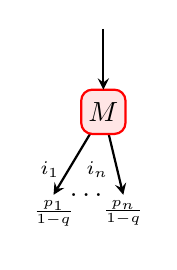
\begin{tikzpicture}[thick,x=18pt,y=15pt,outer sep=0pt,inner sep=2pt]
	\coordinate (m) at (0,0);
	
	\node at (-0.3,-2) {$\dots$};
	
	\begin{scope}[->,>=stealth,anchor=north]
		\draw (m)--node[pos=0.7,anchor=east]{$\termcolor\scriptstyle{i_1\,}$} (-1,-2) node {$\vphantom:\typecolor\scriptstyle{\ifx#11p_1\else\frac{p_1}{1-q}\fi}$};
		\draw (m)--node[pos=0.7,anchor=east]{$\termcolor\scriptstyle{i_n\,}$} (.4,-2) node {$\vphantom:\typecolor\scriptstyle{\ifx#11p_n\else\frac{p_n}{1-q}\fi}$};
	\ifx#11
		\draw (m)--node[pos=0.7,anchor=west]{\,$\termcolor\scriptstyle{j}$}   ( 1,-2) node {$\vphantom:\typecolor\scriptstyle{q}$};
	\fi
	\end{scope}
	
	\node (x) at (0,-3) {};
	
	\coordinate (a) at ( .85,-1.7);% \node[gray,circle,draw,inner sep=0pt,minimum size=2pt] at (a) {};
	\coordinate (b) at (1.25,-1.6);% \node[gray,circle,draw,inner sep=0pt,minimum size=2pt] at (b) {};
	
    	\ifx#10
		%\draw (m) [rounded corners=20pt] -- (1.25,-2.5) [rounded corners=5pt] -- (1.25,1.5) -- (0,1.5) -- (0,1);
		\draw[rounded corners=5pt] (m) -- (.5,-1) .. controls (a) and (b) .. (1.25,-.75) -- (1.25,1.5) -- (0,1.5) -- (0,1);
    	\fi	
	
	\node[draw=red,fill=red!10,rounded corners,minimum size=16pt] (M) at (m) {$\term M$};
	\draw[->,>=stealth] (0,2)--(M);	
\end{tikzpicture}}}
}

%==================================================================================================== FRONTMATTER

\title{Simple Types for Almost Sure Termination}

\author{Ugo {Dal Lago}}{University of Bologna, Italy \and INRIA Sophia Antipolis, France}{ugo.dallago@unibo.it}{https://orcid.org/0000-0001-9200-070X}{}

\author{Willem B. Heijltjes}{University of Bath, United Kingdom \and \url{http://willem.heijltj.es}}{w.b.heijltjes@bath.ac.uk}{https://orcid.org/0009-0001-8941-1150}{}

\authorrunning{U. Dal Lago and W.\,B. Heijltjes}

\Copyright{Ugo Dal Lago and Willem B. Heijltjes}

\ccsdesc[500]{Theory of computation~Lambda calculus}
\ccsdesc[300]{Theory of computation~Probabilistic computation}

\keywords{probabilistic lambda-calculus, type systems, almost sure termination}

%\relatedversion{}

%\acknowledgements{Georgina Majury?}

\nolinenumbers

\EventEditors{}
\EventNoEds{0}
\EventLongTitle{}
\EventShortTitle{}
\EventAcronym{}
\EventYear{}
\EventDate{}
\EventLocation{}
\EventLogo{}
\SeriesVolume{}
\ArticleNo{}

%==================================================================================================== DOCUMENT
\begin{document}

\maketitle

\begin{abstract}

\end{abstract}
   
%---------------------------------------------------------------------------------------------------- INTRODUCTION

\section{Introduction}

We are interested in applying the tools of the $\lambda$-calculus, in particular confluent reduction and type systems, to probabilistic computation. In~\cite{DalLago-Guerreri-Heijltjes-2020} we restored confluence to a probabilistic $\lambda$-calculus, the probabilistic event $\lambda$-calculus (PEL), by decomposing probabilistic choice into a \emph{sampling} construct and a \emph{conditional}. Independently in~\cite{Antonelli-DalLago-Pistone-2022} and~\cite{Heijltjes-Majuri-2025}, from different inspirations we converged on essentially the same probabilistic type system for the PEL to give lower bounds on the probability of termination. In this paper we further extend the calculus, and develop a type system for \emph{almost sure termination} (AST): termination with probability one.

We start from the following observation. \emph{Iteration}, generally represented by while-loops, repeats a given function $f$ until a condition is fulfilled. In the typed case, illustrated  below, the function $f$ is required to return a sum $B+A$ where the choice between returning a value $A$ or $B$ represents the condition. Then $\mathsf{iter}\,f$ first evaluates $f$, and exits on $B$ and repeats on $A$.
\[
\begin{array}{@{}r@{}l@{}}
	f &{}: A \to B+A
\\ \hline
	\mathsf{iter}\,f &{}: A\to B
\end{array}
	%\infer{\mathsf{iter}~f : A\to B} { f : A \to B+A } 
	% \qquad \mathsf{iter}~f~=~[\mathsf{id},\mathsf{iter}~f]\,\circ\,f
	%It is defined as the least solution to the equation below right, where $[-,-]$ is the co-diagonal of the coproduct.
\]
We observe that if we replace $B+A$ by a probabilistic sum $B \oplus_p A$ with a fixed probability $p\in (0,1]$, i.e.\ the probability of choosing $B$ is non-zero, then $\mathsf{iter}\,f$ is \emph{almost surely terminating} (provided of course that $f$ is itself terminating). This opens a way to approach almost sure termination via type systems.

These considerations demonstrate how probabilistic choice is tied up with other imperative features such as sequentiality and iteration. Derived from the PEL, the second author has developed new approach to unifying the $\lambda$-calculus with imperative features, the Functional Machine Calculus (FMC)~\cite{Heijltjes-2022}. Its most recent iteration~\cite{Heijltjes-2025-MFPS} features branching sequential computation and iteration, providing an ideal vehicle for our present study.

In the FMC each branch of the computation is labelled with a \emph{choice} label $i,j,k,\dots$, which takes the role of a constant, an exception, a case label, or an exit status. For example, the boolean constants $\bot$ and $\top$ are choice labels. Iteration of a term $\term M$ is written $\term{M^i}$, which evaluates $\term M$ and repeats if $\term M$ chooses $i$, and terminates for any other choice. The calculus encodes a fair probabilistic choice, which we write as $\term{M+N}$.

\begin{example}
The term $\term{(\bot + (\top + \,i))^i}$ chooses $\bot$ with probability $\frac12$, $\top$ with probability $\frac14$, and iterates with probability $\frac14$, to give an overall probability of $\frac 23$ for $\bot$ and $\frac 13$ for $\top$. We illustrate it pictorially as follows.
\[
	\term{(\bot + (\top + \,i))^i}
\quad=\quad
\vcenter{\hbox{%
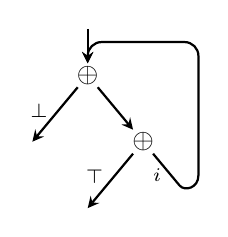
\begin{tikzpicture}[thick,x=20pt,y=24pt,outer sep=0pt,inner sep=1pt]
	\node (x) at (1,2) {$\termcolor\oplus$};
	\node (y) at (2,1) {$\termcolor\oplus$};

	\coordinate (a) at (2.75,0.25); %\node[gray,circle,draw,inner sep=0pt,minimum size=2pt] at (a) {};
	\coordinate (b) at (3   ,0.3);  %\node[gray,circle,draw,inner sep=0pt,minimum size=2pt] at (b) {};
	
	\begin{scope}[->,>=stealth,anchor=north]
	
	\draw (1,2.7)--(x);
	\draw (x)--(y);
	\draw (x) --node[pos=0.6,anchor=south east]{$\termcolor\scriptstyle{\bot}$} (0,1);
	\draw (y) --node[pos=0.6,anchor=south east]{$\termcolor\scriptstyle{\top}$} (1,0);
	
	\draw[rounded corners=5pt] (y) -- node[pos=0.6,anchor=north east]{$\,\termcolor\scriptstyle{i}$}  
	  (2.5,0.5) .. controls (a) and (b) .. (3,0.7) -- (3,2.5) -- (1,2.5) -- (x);
	\end{scope}
\end{tikzpicture}}}
\]
\end{example}

The type system, simplified for this introduction to omit return values, records the probability of terminating with each given choice. A term $\term M$ is typed as follows, indicating that it may choose $i_k$ with probability $p_k$ from choices $i_1$ through $i_n$.
\[
	\term{M : \e ~=>~ p_1 i_1 + \cdots + p_n i_n }
\]
Here, the double arrow $\type{=>}$ is the function type and $\type\varepsilon$ represents the lack of an input value. The return type is a probability (sub-)distribution over the choices $\{i_1,\dots,i_n\}$, written as a formal sum. The probabilities $p_1$ through $p_n$ may sum to less than one, with the remainder representing a probability of divergence.

\begin{example}
For the body of our example term, without the loop, we have the following type.
\[
	\term{\bot + (\top + \,i) : \e ~=>~ /12\bot + /14\top + /14i}
\]
\end{example}

Iteration $\term{M^i}$ removes a choice $i$ from the possible return choices. In the probabilistic setting, the remaining probabilities must then be renormalized to a distribution. That is, if $i$ has probability $q$, the remaining choices (including divergence) have a total probability $1-q$, and must be multiplied by $\frac1{1-q}$ to return the total to one. Typing for iteration is then as follows.
\[
\begin{array}{@{}r@{}l@{}}
	\term{M}   &{}: \type{\e ~=>~ p_1i_1 + \dots + p_ni_n + qj}
\\ \hline \\[-10pt]
	\term{M^j} &{}: \type{\e ~=>~ /{p_1}{1-q}i_1 + \dots + /{p_n}{1-q}i_n}
\end{array}	
\qquad
\term{M}=\looppic1 \qquad \term{M^j}=\looppic0
\]

\begin{example}
The return type for our example term is given by renormalizing the sub-distribution $\type{/12\bot + /14\top}$, remaining after removing the element $\type{/14i}$, by multiplying by $\frac 43$, giving the following.
\[
	\term{(\bot + (\top + \,i))^i : \e ~=>~ /23\bot + /13\top}
\]
\end{example}

Types for iteration then correctly give the probabilities for each choice. Consider $\term{M^j}$ where $j$ has probability $q$ in $\term M$. For any other choice $i$ with probability $p$ in $\term M$ the chance of $\term{M^j}$ choosing $i$ is given by the following geometric series, generated by choosing $i$ immediately, then after one loop, after two loops, and so forth. The limit of this series is the probability given by the type system.
\[
	p + pq + pq^2 + pq^3 + \cdots ~=~ \frac p{1-q}
\]



The typed calculus, the probabilistically typed FMC (FMC$^\oplus$), achieves the following. A term is guaranteed to terminate with the probabilities of its return type, which is almost sure termination if the sum probability is one, also in the presence of higher-order probabilistic functions. In a first-order setting it guarantees \emph{positive} almost sure termination (expected evaluation time is finite), where still it may capture all Markov chains and directly compute their expected output. In the higher-order setting, which gives access to Church numerals, there are examples of \emph{non-positive} or \emph{null} AST.

The FMC$^\oplus$ is a new type system for the FMC~\cite{Heijltjes-2025}, while the underlying calculus remains essentially the same. It is also a conservative extension of the \emph{sequential} probabilistic event $\lambda$-calulculus

%\cite{Hurd-2002}

%while (x>0) { x := x-1 [1/2] x := x+1 }

%  -1 (+) +1 : (=> p1.1 + p2.2 + p3.3 + ...) => (1/2 p1).0 + (1/2 p2).1 + (1/2 p1+p3).2 + (1/2 p2+p3).3 + ...


\bigskip

{\color{green!66!black}

* Conservative extension of [Curry \&\ Howard meet Borel] and [Simple Types for Probabilistic Termination].

* Uses \emph{iteration} rather than \emph{recursion} to obtain probabilistic typeability.

* Probabilistic recursion is difficult as it requires probabilistic function variables at type level, essentially using dependent types. Example: probabilistic Church numerals and Y-combinator.

* Probabilistic iteration is straightforward and natural, taking  $f : A \to A+B$ to $\mathsf{iter}~f : A\to B$, which is AST if $A+B$ is a probabilistic sum which has a non-zero probability of choosing $B$. 


* Zero-th order and first-order fragments.
}

%---------------------------------------------------------------------------------------------------- PROBABILISTIC FMC

\section{The probabilistically-typed FMC}


Terms:
\[
\term{M,N} ~\coloneqq~ \term{x} ~\mid~ \term{<x>.M} ~\mid~ \term{[N].M} ~\mid~ \term{i} ~\mid~ \term{M;i->N} ~\mid~ \term{M^i} ~\mid~ \term{?a.M}
\]

\noindent
Abbreviations:
\[
	\term{M+N} ~=~\term{?a.a;\top->M;\bot->N}
\]

\noindent
Sets of things:
\[
\begin{array}{lll}
	\0,\1   &~\in~\B      & \text{boolean constants}
\\	a,x,y,z &~\in~\Var    & \text{variables}
\\  i,j,k   &~\in~\Choice & \text{choices, where also}~\B\subset\Choice
\\	R,S,T   &~\in~\Stack  & \text{stacks of terms}
\\  L,K     &~\in~\Cont   & \text{continuation stacks: stacks of cases}~\term{i->M}
\\	r,s,t   &~\in~\Trace  & \text{traces: finite sequences of booleans}~\top,\bot
\\  p,q     &~\in~[0,1]   & \text{probabilities}
\end{array}
\]

Machine:
\[
\begin{array}{lc}
	  \mathsf{push}     & \step- t S {[N].M} K             t {S\,\term N} M K
\\ \\ \mathsf{pop}      & \step- t {S\,\term N} {<x>.M} K  t S {\{N/x\}M} K
\\ \\ \mathsf{select}   & \step- t S i {(\term{i->M})\,K}  t S M K
\\ \\ \mathsf{reject}   & \step- t S i {(\term{j->M})\,K}  t S i K
\\ \\ \mathsf{sequence} & \step- t S {M;i->N} K            t S M {(\term{i->N})\,K}
\\ \\ \mathsf{iterate}  & \step- t S {M^i} K               t S M {(\term{i->M^i})\,K}
\\ \\ \mathsf{sample}   & \step- t S {?a.M} K        {t\,\1} S {\{\1/a\}M} K
                   \quad  \step- t S {?a.M} K        {t\,\0} S {\{\0/a\}M} K
\end{array}
\]

A \emph{run} of the machine is a sequence of steps, written with a double line as below. A \emph{successful} run is one terminating in a \emph{final state} $\state tTi\e$ with a choice term $\term i$ and empty continuation stack.
\[ 
	\step= sSMK tTNL
\]

% - - - - - - - - - - - - - - - - - - - - - - - - - - - - - - Big-step semantics
\subsection{Big-step semantics}

A \emph{frontier} $F$ is a set of traces such that no element in $F$ is a prefix of another. A frontier is \emph{total} if it contains a prefix of every stream in $\B^\N$.

To collect the outcomes of evaluating a term, a \emph{return family} $\DS$ in a frontier $F$ assigns to each trace $t\in F$ a pair $(S,\term i)$ of a stack and choice. We write $\floor\DS$ for the frontier $F$ over which $\DS$ is defined.
\[
	\DS,\DT~:~F\to\Stack\times\Choice
\]
The set $\runs SM$ for a stack $S$ and term $\term M$ is the return family that collects the traces and outputs of all successful runs, as follows. Note that this is well-defined as a family over a frontier since each run has a unique trace.
\[
	\runs SM~=~\{~t\mapsto (T,\term i)~\mid~\step= \e SM\e tTi\e~\}
\] 

\emph{Union} of two return families $\DS\cup\DT$ is that of their underlying relations, and is a return family if they are defined over disjoint frontiers, $\floor\DS\cap\floor\DT=\varnothing$. Likewise, \emph{inclusion} between families $\DS\subseteq\DT$ is inclusion as relations, which means $\floor\DS\subseteq\floor\DT$ and $\DS(t)=\DT(t)$ for all $t\in\floor\DS$. We define the following notions below: the \emph{extension} $s\pfx\DS$ of a return family $\DS$ with a trace $s$, its \emph{restriction} $\DS\only i$ to a choice $i$, and its \emph{exclusion} $\DS\less i$ of $i$. 
\[
\begin{array}{l@{}l}
	    s\pfx\DS   &~=~\{ s\,t\mapsto(S,j) \mid t\mapsto(S,j)\in\DS\}
\\[5pt]	\DS\only i &~=~\{ t\mapsto(S,j)\in\DS \mid j=i \} 
\\[5pt]	\DS\less i &~=~\{ t\mapsto(S,j)\in\DS \mid j\neq i \}
\end{array}
\]

\begin{definition}
The \emph{evaluation} relation $\evalarrow$ on terms $\eval SM\DT$ and continuations $\eval\DS{i->M}\DT$ is defined inductively by the following rules.
\[
\begin{array}{@{}c@{\qquad}c@{\qquad}c@{}}
	\infer{\eval Si{\{\e\mapsto (S,i)\}}}{}
&	\infer{\eval {S\,\term N}{<x>.M}\DT}{\eval S{\{N/x\}M}\DT}
&	\infer{\eval R{M;i->N}\DT}{\eval RM\DS && \eval\DS{i->N}\DT}
\\ \\
	\infer{\eval SM\varnothing}{}
&	\infer{\eval S{[N].M}\DT}{\eval {S\,\term N}M\DT}
&	\infer{\eval S{?a.M}{(\0\pfx\DT_0)\cup(\1\pfx\DT_1)}}{\eval S{\{\0/a\}M}{\DT_0} && \eval S{\{\1/a\}M}{\DT_1}}
\\ \\
\multicolumn{2}{@{}c@{\qquad}}{
	\infer{\eval S{M^i}{\sup_{n\in\N}(\DT_n\less i)}}{
    	\eval SM{\DT_0}
    	&& 
    	\{\eval{\DT_n}{i->M}{\DT_{n+1}}\}_{n\in\N}
    }
}&
	\infer{\eval\DS{i->M}{\DS\less i\cup\bigcup_{t\in\floor{\DS\only i}} t\pfx\DT_t}}{ \{\eval {S_t}M{\DT_t}\}_{t\,\mapsto\,(S_t,i)~\in~\DS\only i} } 
\end{array}	
\]
\end{definition}

Observe that the \emph{sample} and \emph{sequence} rules are well-defined as the unions are disjoint, and in the \emph{iterate} rule for $\term{M^i}$ the supremum is well-defined since each $\DT_{n+1}$ is given (in the continuation rule) as $\DT_n\less i\cup\DT'$ for some $\DT'$, so that we immediately have $\DT_n\less i\subseteq\DT_{n+1}\less i$.



% - - - - - - - - - - - - - - -
\begin{proposition}
\label{prop:eval-run}
If $\eval SM\DT$ then $\DT~\subseteq~\runs SM$.
\end{proposition}

\begin{proof}
By induction on the derivation for $\eval SM\DT$.
\begin{itemize}

	% Choice
	\item \emph{Choice:}
\[
	\infer{\eval Si{\D{\e\mapsto (S,i)}}}{}
\]
The only run for the state $(\e,S,\term i,\e)$ is the empty run, which gives the singleton $\runs SM=\{\e\mapsto (S,i)\}$ as required.

	% Fail
	\item \emph{Fail:}
\[
	\infer{\eval SM\varnothing}{}
\]
It is immediate that $\varnothing\subseteq\runs SM$.

	% Pop
	\item \emph{Pop:}
\[
	\infer{\eval {S\,\term N}{<x>.M}\DT}{\eval S{\{N/x\}M}\DT}
\]
Since a run for $\state \e{S\,\term N}{<x>.M}\e$ must necessarily start with a $\mathsf{pop}$ transition to $\state\e S{\{N/x\}M}\e$, we have:
\[
	\runs{S\,\term N}{<x>.M}~=~\runs S{\{N/x\}M}
\]
The case is then immediate by induction.

	% Push
	\item \emph{Push:}
\[
	\infer{\eval S{[N].M}\DT}{\eval {S\,\term N}M\DT}
\]
Since a run for $\state \e S{[N].M}\e$ must necessarily start with a $\mathsf{push}$ transition to $\state\e{S\,\term N}M\e$, we have:
\[
	\runs S{[N].M}~=~\runs{S\,\term{N}}M
\]
The case is then immediate by induction.

	% Sequence
	\item \emph{Sequence:}
\[
	\infer{\eval R{M;i->N}\DT}{\eval RM\DS && \eval\DS{i->N}\DT}
\qquad
	\infer{\eval\DS{i->M}{\DS\less i\cup\bigcup_{t\in\floor{\DS\only i}} t\pfx\DT_t}}{ \{\eval {S_t}M{\DT_t}\}_{t\,\mapsto\,(S_t,i)~\in~\DS\only i} }
\]
Let $s\mapsto (T,j)\in\DT$ as above left, where $\DT=\DS\less i\cup\bigcup_{t\in\floor{\DS\only i}} t\pfx\DT_t$ as above right. It must be shown that $s\mapsto (T,j)\in\runs R{M;i->N}$. There are two cases.

\begin{itemize}
	\item $s\mapsto(T,j)\in\DS\less i$. Then $j\neq i$ and by induction on $\eval RM\DS$ we have $s\mapsto(T,j)\in\runs RM$, which means there is a run as below left. This gives the run below right, which shows $s\mapsto(T,j)\in\runs R{M;i->N}$.
\[
	\step= \e RM\e tTj\e
\qquad\qquad	    	
    \begin{array}{@{(~}l@{~,~}l@{~,~}r@{~,~}r@{~)}}
    	      \e & R & \term{M;i->N} & \e
    \\ \hline \e & R & \term{M}      & (\term{i->N})
    \\ \dline  s & T & \term{j}      & (\term{i->N})
    \\ \hline  s & T & \term{j}      & \e
    \end{array}
\]

	\item $s\mapsto(T,j)\in\bigcup_{t\in\floor{\DS\only i}} t\pfx\DT_t$. Then there is some $t\mapsto(S,i)\in\DS\only i$ such that $s = t\,t'$ and $t'\mapsto(T,j)\in\DT_t$. By induction, $t\mapsto(S,i)\in\runs RM$ and $t'\mapsto(T,j)\in\runs SN$. This gives the two runs below left, from which that below right is then constructed, showing that $s\mapsto(T,j)\in\runs R{M;i->N}$.
\[
	\begin{array}{@{}c@{}}
		\step= \e RM\e tSi\e
	\\ \\
		\step= \e SN\e{t'}Tj\e
	\end{array}
\qquad\qquad
    \begin{array}{@{(~}l@{~,~}l@{~,~}r@{~,~}r@{~)}}
    	      \e    & R & \term{M;i->N} & \e
    \\ \hline \e    & R & \term{M}      & (\term{i->N})
    \\ \dline t     & S & \term{i}      & (\term{i->N})
    \\ \hline t     & S & \term{N}      & \e
    \\ \dline t\,t' & T & \term{j}      & \e
    \end{array}
\]
\end{itemize}

	% Sample
	\item \emph{Sample:}
\[
	\infer{\eval S{?a.M}{(\0\pfx\DT_0)\cup(\1\pfx\DT_1)}}{\eval S{\{\0/a\}M}{\DT_0} && \eval S{\{\1/a\}M}{\DT_1}}
\]
Let $t\mapsto(T,i)\in\0\pfx\DT_0\cup\1\pfx\DT_1$. Then either $t=\0\,s$ and $s\mapsto(T,i)\in\DT_0$, for some $s$, or $t=\1\,s$ and $s\mapsto(T,i)\in\DT_1$. We consider the case $t=\0\,s$; the other is analogous. By induction we have the run below left, which then gives that below right, showing that $t\mapsto(T,i)\in\runs S{?a.M}$.
\[
	\step= \e S{\{\0/a\}M}\e sTi\e 
\qquad\qquad
    \begin{array}{@{(~}l@{~,~}l@{~,~}r@{~,~}r@{~)}}
    	      \e    & S & \term{?a.M}      & \e
    \\ \hline \0    & S & \term{\{\0/a\}M} & \e
    \\ \dline \0\,s & T & \term{i}         & \e
    \end{array}
\]

	% Iterate
	\item \emph{Iterate:}
\[
	\infer{\eval S{M^i}{\sup_{n\in\N}(\DT_n\less i)}}{
    	\eval SM{\DT_0}
    	&& 
    	\{\eval{\DT_n}{i->M}{\DT_{n+1}}\}_{n\in\N}
    }
\qquad
	\infer{\eval\DS{i->M}{\DS\less i\cup\bigcup_{t\in\floor{\DS\only i}} t\pfx\DT_t}}{ \{\eval {S_t}M{\DT_t}\}_{t\,\mapsto\,(S_t,i)~\in~\DS\only i} } 
\]
First, by induction on $n$ it will be shown that if $t\mapsto(T,j)\in\DT_n$ then there is a run:
\[
	\step= \e S{M^i}\e tTj{\term{i -> M^i}} 
\]
For $n=0$, by the inductive hypothesis for $\eval SM{\DT_0}$ and $t\mapsto(T,j)\in\DT_0$ we have the run below left, which then gives that below right.
\[
	\step= \e SM\e tTj\e 
\qquad	
    \begin{array}{@{(~}l@{~,~}l@{~,~}r@{~,~}r@{~)}}
    	      \e & S & \term{M^i} & \e
    \\ \hline \e & S & \term{M}   & (\term{i->M^i})
    \\ \dline  t & T & \term{j}   & (\term{i->M^i})
    \end{array}
\]
For the case $n+1$, by the inductive hypothesis for $\eval{\DT_n}{i->M}{\DT_{n+1}}$ and $t\mapsto(T,j)\in\DT_{n+1}$ we have two cases: $t\mapsto(T,j)$ is either in $\DT_n\less i$ or in $\bigcup_{t\in\floor{\DT_n\only i}} t\pfx\DT_t$. The former case is immediate by the inductive hypothesis. In the latter case, $t=r\,s$ and there are $R$ and $\DT_s$ such that
\[
	r\mapsto(R,i)\in\DT_n
\qquad
	\eval RM{\DT_s}
\qquad
	s\mapsto(T,j)\in\DT_s
\]
The first statement gives the first run below left, by the induction on $n$, and the induction on the latter two statements gives the second. Then the required run is given below right.
\[
	\begin{array}{@{}c@{}}
		\step= \e S{M^i}\e rRi{(\term{i->M^i})}
	\\ \\
		\step= \e RM\e sTj\e
	\end{array}
\qquad\qquad
    \begin{array}{@{(~}l@{~,~}l@{~,~}r@{~,~}r@{~)}}
    	      \e    & S & \term{M^i} & \e
    \\ \dline r     & R & \term{i}   & (\term{i->M^i})
    \\ \hline r     & R & \term{M^i} & \e
    \\ \hline r     & R & \term{M}   & (\term{i->M^i})
    \\ \dline r\,s  & T & \term{j}   & (\term{i->M^i})
    \end{array}
\]

For the overall case, let $t\mapsto(T,j)\in\sup_{n\in\N}(\DT_n\less i)$. Then there is some $m$ such that $t\mapsto(T,j)$ is in $\DT_m\less i$. By the above, and since $i\neq j$, we have the following run, which shows that $t\mapsto(T,j)\in\runs S{M^i}$.
\[
    \begin{array}{@{(~}l@{~,~}l@{~,~}r@{~,~}r@{~)}}
    	      \e & S & \term{M^i} & \e
    \\ \dline  t & T & \term{j}   & (\term{i->M^i})
    \\ \hline  t & T & \term{j}   & \e
    \end{array}
\]

\end{itemize}
\end{proof}
% - - - - - - - - - - - - - - -



{\color{green!66!black} The following is not essential but could be nice. Seems a bit of work, though.}

\begin{proposition}
$\eval SM{\runs SM}$.
\end{proposition}




%---------------------------------------------------------------------------------------------------- TYPES

\section{Types}


Types will use \emph{indexed probability (sub-)distributions}, which are families over finite sets of choices $I,J$.

\noindent
Types:
\[
\begin{array}{lr@{~\coloneqq~}l}
	\text{types}	   & \type{s,t} & \type{!s => !tI}
\\	\text{stack types} & \type{!t}  & \type{t_1..t_n}
\\  \text{sum types}   & \type{!tI} & \type{\{!t_i.p_i\}_{i\in I}}~\quad~\sum_{i\in I}p_i\leq 1
\end{array}
\]

\noindent
Definitions:
\[
\begin{array}{l@{}ll}
		\type{(!t.p)_i}    &~=~ \type{\{!t_i.p_i\}_{\{i\}}}                       & \text{where~}\type{!t_i}=\type{!t},~p_i=p
\\[5pt] \type{!sI + !tJ}   &~=~ \type{!sI \cup !tJ}                               & \text{if~}(I\cap J=\varnothing)
\\[5pt] \type{!s\,!tI}     &~=~ \type{\{!s\,!t_i . p_i \mid !t_i.p_i \in !tI\}}
\\[5pt]	\type{q.!tI}       &~=~ \type{\{ !t_i . q\,p_i \mid  !t_i.p_i \in !tI\}}
\\[5pt]	\type{!tI-J}       &~=~ \type{\{ !t_i.p_i \in !tI \mid i\notin `J\}}
\\[5pt] \type{!tI|J}       &~=~ \type{\{ !t_i.p_i \in !tI \mid i\in `J\}}
\\[5pt] \type{!sI ++ !tJ}  & \multicolumn{2}{@{}l@{}}{~=~ \type{\{!t_i . p_i+q_i \mid !t_i.p_i \in !sI|J~`,~!t_i.q_i\in!tJ|I\}}}
\\[5pt]                    &\quad\type{\cup~(!sI-J)~\cup~(!tJ-I)}                 & \text{if~} \forall i\in(I\cap J).~\type{s_i}=\type{t_i}
\end{array}
\]

%\[
%\begin{array}{lr@{~\coloneqq~}l}
%	\text{types}	   & \type{s,t} & \type{!s => !tI}
%\\	\text{stack types} & \type{!t}  & \type{t_1..t_n}
%\\  \text{sum types}   & \type{!tI} & \type{\{i \mapsto !t_i.p_i\}_{i\in I}}~\quad~\sum_{i\in I}p_i\leq 1
%\end{array}
%\]
%
%\noindent
%Definitions:
%\[
%\begin{array}{lll}
%		\type{i(!t.p)}     &~=~ \type{\{i \mapsto !t.p\}}
%\\[5pt] \type{!sI ++ !tJ}  &~=~ \type{!sI \cup !tJ} \qquad (I\cap J=\varnothing)
%\\[5pt] \type{!s\,!tI}     &~=~ \type{\{i\mapsto !s\,!t_i . p_i \mid i\mapsto !t_i.p_i \in !tI\}}
%\\[5pt]	\type{q.!tI}       &~=~ \type{\{i\mapsto  !t_i . q\,p_i \mid i\mapsto !t_i.p_i \in !tI\}}
%\\[5pt]	\type{!tI-J}       &~=~ \type{\{i\mapsto !t_i.p_i \in !tI \mid i\notin J\}}
%\\[5pt] \type{!tI|J}       &~=~ \type{\{i\mapsto !t_i.p_i \in !tI \mid i\in J\}}
%\\[5pt] \floor{\type{!tI}} &~=~ \{ i\mapsto \type{!t_i}\}_{i\in I}
%\\[5pt] \type{!sI + !tJ}   &~=~ \type{\{i\mapsto !t_i . p_i+q_i \mid i\mapsto !t_i.p_i \in !sI|J~`,~i\mapsto !t_i.q_i\in!tJ|I\}}
%\\                         &\qquad \type{~\cup~(!sI-J)~\cup~(!tJ-I)} 
%%\\[5pt] \type{!sI + !tI}   &~=~ \type{\{i\mapsto !t_i.p_i+q_i \mid i\mapsto !t_i.p_i \in !sI,~i\mapsto !t_i.q_i\in !tI \}} & \floor{\type{!sI}}=\floor{\type{!tI}}
%%\\[5pt] \type{!sI + !tJ}   &~=~ \type{(!sI|J v !tJ|I) u (!sI-J) u (!tJ-I)}
%\end{array}
%\]

\noindent
Typing rules:
\[
\begin{array}{lc}
      \mathsf{variable}  & \infer{\term{G, x:t |- x:t}}{}
\\ \\ \mathsf{expansion} & \infer{\term{G |- M: !s\,!r => !r\,!tI}}{\term{G |- M: !s => !tI}}
\\ \\ \mathsf{push}      & \infer{\term{G |- [N].M : !s => !tI}}{\term{G |- N:r} && \term{G |- M : r\,!s => !tI}}
\\ \\ \mathsf{pop}       & \infer{\term{G |- <x>.M : r\,!s => !tI}}{\term{G , x:r |- M: !s => !tI}}
\\ \\ \mathsf{choice}    & \infer{\term{G |- i: !s => (!s.1)_i}}{}
\\ \\ \mathsf{sequence}  & \infer{\term{G |- M;i->N : !r => !sI ++ (p . !tJ)}}
                                 {\term{G |- M: !r => !sI + (!s.p)_i} && 
                                  \term{G |- N: !s => !tJ}}
\\ \\ \mathsf{iterate}   & \infer{\term{G |- M^i: !s => /1{1-p} . !tI}}{\term{G |- M: !s => !tI + (!s.p)_i} && (p\neq 1)}
\\ \\ \mathsf{sample}    & \infer{\term{G |- ?a.M : !r => (/12 . !sI) ++ (/12 . !tJ)}}{\term{G , a: \e => (\e.1)_\bot |- M: !r => !sI} && \term{G , a: \e => (\e.1)_\top |- M: !r => !tJ}}
\\ \\ \mathsf{zero}      & \infer{\term{G |- M : !s => 0 . !tI}}{}
\end{array}
\]



% - - - - - - - - - - - - - - - - - - - - - - - - - - - - - - Runnability
\newpage
\subsection{Runnability}

The \emph{probability} of a trace $t$ is $p(t)=(\fraction12)^{|t|}$ where $|t|$ is the \emph{length} of $t$.

\[
\begin{array}{l@{}l}
%	     |\DS|       &~=~ \sum_{t\in\floor\DS}~p(t)
%\\[5pt]
         |\DS|_i     &~=~ \sum_{t\in\floor{\DS\only i}}~p(t)
\\[5pt]  \floor\DS_i &~=~ \{ S \mid t\mapsto(S,i)\in\DS \}
\end{array}
\]

\begin{definition}
The set $\RUN{t}$ of \emph{runnable terms} for a type $\type t$ is defined as the set of closed terms
\[
	\RUN{!s => !tI} = \{ \term M ~\mid~ \forall S \in\RUN{!s}.~\exists\DT\in\RUN{!tI}.~\eval SM\DT~\}
\]
where the runnable sets for stack types $\type{!t}$ and sum types $\type{!tI}$ are as follows.
\[
    \RUN{t_1..t_n} = \{ \e\,\term{M_1}\dots \term{M_n} \mid \term{M_i}\in\RUN{t_i} \}
\]
\[
	\RUN{\{!t_i.p_i\}_{i\in I}} = \{ \DT \mid \forall i\in I.~\floor\DT_i\subseteq\RUN{!t_i}~\wedge~|\DT|_i\geq p_i~\}
\]
\end{definition}



% - - - - - - - - - - - - - - - 
\begin{lemma}
\label{lem:run-union}
If $\DS\in\RUN{!sI}$ and $\DT\in\RUN{!tJ}$ then $\DS\cup\DT\in\RUN{!sI ++ !tJ}$ if $\DS\cup\DT$ and $\type{!sI++!tJ}$ are defined.
\end{lemma}

\begin{proof}
Let $\type{!sI}=\type{\{!s_i.p_i\}_{i\in I}}$ and $\type{!tJ}=\type{\{!t_j.q_j\}_{j\in J}}$. Note that $\DS\cup\DT$ is defined if $\floor\DS\cap\floor\DT=\varnothing$, and $\type{!sI++!tJ}$ if $\type{!s_i}=\type{!t_i}$ for all $i\in I\cap J$. We need to show two properties.
\begin{itemize}
	 \item[1)] If $t\mapsto(S,i)\in\DS\cup\DT$ then $S\in\RUN{!s_i}$ if $i\in I$ and $S\in\RUN{!t_i}$ if $i\in J$. This is as follows: since $\DS\in\RUN{!sI}$, if $t\mapsto(S,i)\in\DS$ then $S\in\RUN{!s_i}$, and since $\DT\in\RUN{!tJ}$, if $t\mapsto(S,i)\in\DT$ then $T\in\RUN{!t_j}$.
	 
	 \item[2)] For $i\in I\cup J$, the probability $|\DS\cup\DT|_i$ is at least: $p_i+q_i$ if $i\in I\cap J$, $p_i$ if $i\in I\less J$, and $q_i$ if $i\in J\less I$. This is as follows: first, $|\DS\cup\DT|_i=|\DS|_i+|\DT|_i$, since both are the sum over those $p(t)$ such that $t\in\floor{\DS\only i}$ or $t\in\floor{\DT\only i}$. Then since $\DS\in\RUN{!sI}$ the probability $|\DS|_i\geq p_i$ for $i\in I$, and since $\DT\in\RUN{!tJ}$ the probability $|\DT|_i\geq q_i$ for $i\in J$.
\end{itemize}
\end{proof}
% - - - - - - - - - - - - - - -



For a context $\Gamma=\term{x_1:t_1,..,x_n:t_n}$ the set $\SRUN{G}$ is a set of substitution maps $\mu$ that assigns each $x_i$ a runnable term $\term M\in\RUN{t_i}$.
\[
	\SRUN{G}~=~\{ \mu \mid \forall\term{x:t}\in\Gamma.~\term{\mu x}\in\RUN{t}\}
\]



% - - - - - - - - - - - - - - -
\begin{lemma}
\label{lem:run}
If $\term{G |- M:t}$ and $\mu\in\SRUN{G}$ then $\term{\mu M}\in\RUN{t}$.
\end{lemma}

\begin{proof}

By induction on the typing derivation.
\begin{itemize}

	% Variable
	\item \emph{Variable:} 
\[
	\infer{\term{G, x:t |- x:t}}{}
\]
By the definition of $\SRUN{G}$ we have $\term{\mu x}\in\RUN t$.

	% Choice
	\item \emph{Choice:}
\[
\infer{\term{G |- i: !s => (!s.1)_i}}{}
\]
Given $S\in\RUN{!s}$ we have $\eval Si\DT$ where $\DT={\{\e\mapsto(S,i)\}}$. Then $\floor\DT_i=\{S\}\subseteq\RUN{!s}$ and $|\DT|_i=p(\e)=1$, which gives $\DT\in\RUN{(!s.1)_i}$, and hence $\term{\mu i}=\term i\in\RUN{!s=>(!s.1)_i}$.

	% Zero
	\item \emph{zero}
\[
\infer{\term{G |- M : !s => 0 . !tI}}{}
\]
We have $\eval S{\mu M}\varnothing$ for any $S$ and $\mu$, and $\varnothing\in\RUN{0.!tI}$ since $\floor\varnothing_i=\varnothing\subseteq\RUN{!t_i}$ and $|\varnothing|_i\geq 0$ for all $i$.

	% Expansion
	\item \emph{Expansion:}
\[
\infer{\term{G |- M: !s\,!r => !r\,!tI}}{\term{G |- M: !s => !tI}}
\]
Let $R\in\RUN{!r}$, $S\in\RUN{!s}$, and $\mu\in\SRUN{G}$. By induction $\eval S{\mu M}\DT$ for some $\DT\in\RUN{!tI}$. Then by induction on the evaluation relation, $\eval{RS}{\mu M}{R\DT}$ where $R\DT=\{ t \mapsto (RT,i) \mid t\mapsto (T,i)\in\DT\}$. Since $R\in\RUN{!r}$ it follows by the definition of $\RUN{!tI}$ that $R\DT\in\RUN{!r\,!tI}$.

	% Push
	\item \emph{Push:} 
\[
\infer{\term{G |- [N].M : !s => !tI}}{\term{G |- N:r} && \term{G |- M : r\,!s => !tI}}
\]
Let $S\in\RUN{!s}$ and $\mu\in\SRUN{G}$. By induction $\term{\mu N}\in\RUN{r}$ and $\term{\mu M}\in\RUN{r\,!s=>!tI}$, where by definition we get $\eval{S\,\term{\mu N}}{\mu M}\DT$ for some $\DT\in\RUN{!tI}$. By the definition of evaluation we get $\eval{S}{[\mu N].\mu M}\DT$ so that we have $\term{[\mu N].\mu M}=\term{\mu([N].M)}\in\RUN{!s=>!tI}$. 

	% Pop
	\item \emph{Pop:}
\[
\infer{\term{G |- <x>.M : r\,!s => !tI}}{\term{G , x:r |- M: !s => !tI}}
\]
Let $S\in\RUN{!s}$, $\term N\in\RUN r$, and $\mu\in\SRUN{G}$. Let $\mu'=\mu\{\term N/x\}$, the substitution map that sends $x$ to $\term N$ and every other variable $y$ to $\mu y$, so that $\mu'\in\SRUN{G,x:r}$. By induction $\eval S{\mu'M}\DT$ for some $\DT\in\RUN{!tI}$, and since $\term{\mu'M}=\term{\mu(\{N/x\}M)}$ by the definition of evaluation $\eval{S\,\term N}{\mu(<x>.M)}\DT$. It follows that $\term{\mu(<x>.M)}\in\RUN{r\,!s=>!tI}$.

	% Sample
	\item \emph{Sample:}
\[
\infer{\term{G |- ?a.M : !r => (/12 . !sI) ++ (/12 . !tJ)}}{\term{G , a: \e => (\e.1)_\0 |- M: !r => !sI} && \term{G , a: \e => (\e.1)_\1 |- M: !r => !tJ}}
\]
Let $R\in\RUN{R}$ and $\mu\in\SRUN{G}$. Let $\mu_0=\mu\{\term\0/a\}$ and $\mu_1=\mu\{\term\1/a\}$, so that $\mu_0\in\SRUN{G , a: \e => (\e.1)_\0}$ and $\mu_1\in\SRUN{G , a: \e => (\e.1)_\1}$. By induction $\eval R{\mu_0M}{\DT_0}$ and $\eval R{\mu_1M}{\DT_1}$ where $\DT_0\in\RUN{!sI}$ and $\DT_1\in\RUN{!tJ}$. We have the following evaluation.
\[
\infer{\eval S{\mu(?a.M)}{(\0\pfx\DT_0)\cup(\1\pfx\DT_1)}}{\eval S{\mu\{\0/a\}M}{\DT_0} && \eval S{\mu\{\1/a\}M}{\DT_1}}
\]
Since $\0\pfx\DT_0$ extends every trace in $\DT_0$ by $\bot$, it multiplies every probability $|\DT_0|_i$ by $\fraction 12$, so that we have $\0\pfx\DT_0\in\RUN{/12.!sI}$. Likewise we have $\1\pfx\DT_1\in\RUN{/12.!tJ}$. Then by Lemma~\ref{lem:run-union}
$(\0\pfx\DT_0)\cup(\1\pfx\DT_1)\in\RUN{(/12 . !sI) ++ (/12 . !tJ)}$ and hence $\term{\mu(?a.M)}\in\RUN{!r => (/12 . !sI) ++ (/12 . !tJ)}$.

	% Continuation
	\item \emph{Continuation:}
As a lemma for the remaining two cases, it will be shown that if $\DS\in\RUN{!sI + (!s.p)_i)}$ and $\term{M}\in\RUN{!s => !tJ}$ then $\eval\DS{i->M}\DT$ for some $\DT\in\RUN{!sI ++ (p . !tJ)}$. By definition, for every $t\mapsto(S_t,i)\in\DS$ we have $S_t\in\RUN{!s}$, and by induction $\eval{S_t}M{\DT_t}$ for some $\DT_t\in\RUN{!tJ}$. Evaluation is then as follows.
\[
\infer{\eval\DS{i->M}{\DS\less i\cup\bigcup_{t\in\floor{\DS\only i}} t\pfx\DT_t}}{ \{\eval {S_t}M{\DT_t}\}_{t\,\mapsto\,(S_t,i)~\in~\DS\only i} } 
\]
Let $\DT=\bigcup_{t\in\floor{\DS\only i}}t\pfx\DT_t$. Since $\DT_t\in\RUN{!tJ}$ and prefixing each trace in $\DT_t$ with $t$ multiplies each probability $|\DT_t|_i$ by $p(t)$, we have $t\pfx\DT_t\in\RUN{p(t).!tJ}$. Then since $|\DS|_i=\sum\{p(t)\mid t\in\floor{\DS\only i}\}\geq p$ we have $\DT\in\RUN{p.!tJ}$. By Lemma~\ref{lem:run-union} then $\DS\less i\cup\DT\in\RUN{!sI ++ (p.!tJ)}$.

	% Sequence
	\item \emph{Sequence:} 
\[
\infer{\term{G |- M;i->N : !r => !sI ++ (p . !tJ)}}
      {\term{G |- M: !r => !sI + (!s.p)_i} && 
       \term{G |- N: !s => !tJ}}
\]
Let $R\in\RUN{!r}$ and $\mu\in\SRUN{G}$. By induction we have $\eval R{\mu M}\DS$ where $\DS\in\RUN{!sI+(!s.p)_i}$. By the \emph{continuation} case above, $\eval\DS{i->\mu N}\DT$ for some $\DT\in\RUN{!sI ++ (p . !tJ)}$. The case then follows by the evaluation below, which gives that $\term{\mu(M;i->N)}\in\RUN{!r => !sI ++ (p . !tJ)}$
\[
	\infer {\eval R{\mu M;i->\mu N}\DT} {\eval R{\mu M}\DS && \eval\DS{i->\mu N}\DT}
\]

	% Iterate
	\item \emph{Iterate:}
\[
\infer{\term{G |- M^i: !s => /1{1-p} . !tI}}{\term{G |- M: !s => !tI + (!s.p)_i} && (p\neq 1)}
\]
Let $S\in\RUN{!s}$ and $\mu\in\SRUN{G}$ so that by induction $\eval S{\mu M}{\DT_0}$ for some $\DT_0\in\RUN{!tI + (!s.p)_i}$. By induction on $n$, using the \emph{continuation} case above, there are $\DT_n$ for all $n\in\N$ where $\eval{\DT_n}{i->\mu M}{\DT_{n+1}}$, with the following evaluation.
\[
\infer{\eval S{\mu M^i}{\sup_{n\in\N}(\DT_n\less i)}}{
    	\eval S{\mu M}{\DT_0}
    	&& 
    	\{\eval{\DT_n}{i->\mu M}{\DT_{n+1}}\}_{n\in\N}
    }
\]
Let $p_n=\sum_{m\leq n}p^m$. By induction on $n$ we have 
\[
	\DT_n\in\RUN{(p_n\cdot !tI) + p^n\cdot (!s.p)_i)}
\] 
as follows. For $n=0$ we have $\DT_0\in\RUN{!tI + (!s.p)_i}$, and for $n+1$ we have
\[
	\type{(p_n . !tI) + p^n . (p . (!tI + (!s.p)_i)))}
	~=~
	\type{(p_{n+1} . !tI)+p^{n+1}.(!s.p_i)} 
\]
so that by the \emph{continuation} case $\DT_{n+1}\in\RUN{(p_{n+1} . !tI)+p^{n+1}.(!s.p_i)}$. Since $i\notin I$ we have $\DT_n\less i\in\RUN{p_n.!tI}$, and since $\{p_n\mid n\in\N\}$ is a geometric series with limit $\fraction 1{1-p}$ we have that $\sup_{n\in\N}(\DT_n\less i)\in\RUN{/1{1-p}.!tI}$ and $\term{\mu M^i}\in\RUN{/1{1-p}!tI}$.
\end{itemize}
\end{proof}
% - - - - - - - - - - - - - - -


Let $|\type{!tI}|=\sum\{ p_i \mid \type{!t_i.p_i} \in \type{!tI} \}$ and $|\DT|=\sum\{ p(t)\mid t\in\floor\DT\}$. 


% - - - - - - - - - - - - - - -
\begin{theorem}[Almost-sure termination]
If $\term{|- M: \e => !tI}$ then $\term M$ almost-surely terminates with probability $|\type{!tI}|$.
\end{theorem}

\begin{proof}
Let $\type{!tI}=\type{\{!t_i.p_i\}_{i\in I}}$. By Lemma~\ref{lem:run} we have $\eval\e M\DT$ with $\DT\in\RUN{!tI}$, which means that $|\DT|_i\geq p_i$ for every $i\in I$, so that $|\DT|\geq|\type{!tI}|$. By Proposition~\ref{prop:eval-run} $\DT\subseteq\runs\e M$, so that $|\runs\e M|\geq|\type{!tI}|$.
\end{proof}
% - - - - - - - - - - - - - - -


\newpage
%----------------------------------------------------------------------------------------------------
\section{Properties of the calculus}

{\color{green!66!black}
Give 0th- and 1st-order fragments, encode Markov chains, show PAST and NAST.
}

%----------------------------------------------------------------------------------------------------
\subsection{Encoding Markov chains}

A Markov chain
\[
	C~=~(S,~s\in S,~F\subseteq S,~\delta:S\less F\to\DD{S})
\]
is given by a set of \emph{states} $S$, a \emph{starting state} $s$, a set of \emph{final states} $F$, and a stochastic transition function $\delta$ from non-final states to states.

\newcommand\sem[1]{\llbracket#1\rrbracket}

The interpretation $\sem C$ of a Markov chain as a term is given as follows. For $C$ as above and $t\in S\less\{s\}$, let
\[
	C(t)~=~(S,~t,~F\cup\{s\},~\delta\less\{s\})
\]
where $\delta\less X$ is the transition function $\delta$ restricted to the domain $\mathrm{dom}(\delta)\less X$. For a distribution of terms
\[
	\DM~=~\D{{\term{M_1}}.p_1,..,{\term{M_n}}.p_n}
\]
let the term $\term{\lfloor\DM\rfloor}$ be the internalization of that distribution:
\[
	\lfloor\D{{\term{M}}.1}\rfloor~=~\term{M} 
\qquad\qquad
	\lfloor\D{{\term{M}}.p}+\DM\rfloor~=~\term{?a_p.a ; \top-> M; \bot -> \lfloor{\fraction1{1-p}}\cdot\DM\rfloor} 
\]
Then the interpretation of a Markov chain $C$ as a term is as follows, where final states are \emph{choices}.
\[
	\sem C~=~
	\left\{\begin{array}{ll}
		\term{s} & \text{if}~s~\in~F
	\\	{\termcolor\lfloor\D{{\sem{C(t_1)}}.p_1,..,{\sem{C(t_n)}}.p_n}\rfloor^s} & \text{where}~\delta(s)=\D{t_1.p_1,..,t_n.p_n}	
	\end{array}\right.
\]
That is, for a non-final state $s$ we inductively translate all children $t$ of $s$ as $\sem{C(t)}$, taking the chain $C(t)$ where $s$ now as a final state and $t$ the new initial state. The term for $C$ is then a term for the distribution $\delta(s)$, with the translation $\sem{C(t)}$ for each child $t$, looping on $s$.

\paragraph{Example}
Consider the following Markov chain $C$, where each arrow has probability $\frac13$.
\[
\vcenter{\hbox{
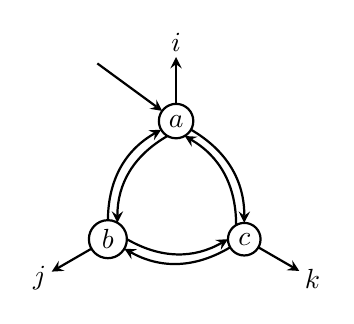
\begin{tikzpicture}[inner sep=2pt,outer sep=0pt,thick]
	\node[circle,draw] (a) at ( 90:1) {$a$} ;
	\node[circle,draw] (b) at (210:1) {$b$} ;
	\node[circle,draw] (c) at (330:1) {$c$} ;
	\node (i) at ( 90:2) {$i$} ;
	\node (j) at (210:2) {$j$} ;
	\node (k) at (330:2) {$k$} ;
	\begin{scope}[->,>=stealth]
	\draw (a.240) to[bend right] (b.60) ;
	\draw (b.0)   to[bend right] (c.180) ;
	\draw (c.120) to[bend right] (a.300) ;
	\draw (a.330) to[bend left]  (c.90) ;
	\draw (b.90)  to[bend left]  (a.210) ;
	\draw (c.210) to[bend left]  (b.330) ;
	\draw (a)--(i);
	\draw (b)--(j);
	\draw (c)--(k);
	\draw (120:2)--(a);
	\end{scope}
\end{tikzpicture}}}
\qquad
\begin{array}{l@{}l@{}l}
	S &~=~& \{a,b,c,i,j,k\}
\\[3pt]	s &~=~& a
\\[3pt]	F &~=~& \{i,j,k\}
\\[3pt]	\delta &~=~&  a \mapsto \D{~b./13~,~c./13~,~i./13~}
\\[3pt]            && b \mapsto \D{~a./13~,~c./13~,~j./13~}
\\[3pt]            && c \mapsto \D{~a./13~,~b./13~,~k./13~}
\end{array}
\]
Its interpretation is as follows, writing $\term{M+N+P}$ for the term $\termcolor\lfloor\D{M./13,N./13,P./13}\rfloor$.
\[
\begin{aligned}
	\sem C &~=~ \term{({\sem{C(b)}}+{\sem{C(c)}}+i)^a}
\\	       &~=~ \term{((a+{\sem{C(b)(c)}}+j)^b + (a+{\sem{C(c)(b)}}+k)^c+i)^a}
\\         &~=~ \term{((a+(a+b+k)^c+j)^b + (a+(a+c+j)^b+k)^c+i)^a}
\end{aligned}
\]
This term is typed as follows. As in the introduction, for brevity we omit return stacks from the types.
\[
\begin{aligned}
	    \term{(a+b+k)^c}         &: \type{\e => /13a + /13b + /13k}
\\[5pt]	\term{ a+(a+b+k)^c+j}~~~ &: \type{\e => /49a + /19b + /19k + /13j}
\\[5pt] \term{(a+(a+b+k)^c+j)^b} &: \type{\e => /12a + /18k + /38j}
\\[5pt] \term{(a+(a+c+j)^b+k)^c} &: \type{\e => /12a + /18j + /38k}
\\[5pt] \term{ (a+(a+b+k)^c+j)^b + (a+(a+c+j)^b+k)^c+i}~~~ &: \type{\e => /13a + /16k + /16j + /13i}
\\[5pt] \term{((a+(a+b+k)^c+j)^b + (a+(a+c+j)^b+k)^c+i)^a} &: \type{\e => /14k + /14j + /12i}
\end{aligned}
\]
The interpretation may be illustrated as follows, where the solid edges represent the tree-shape of the probabilistic sums, while the dashed edges represent the loops.
\[
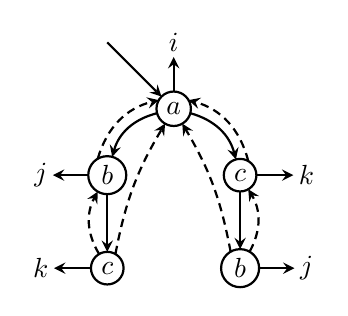
\begin{tikzpicture}[x=24pt,y=-24pt,inner sep=2pt,outer sep=0pt,thick]
	\node[circle,draw] (a) at (1,0) {$a$};
	\node[circle,draw] (b) at (0,1) {$b$};
	\node[circle,draw] (c) at (2,1) {$c$};
	\node[circle,draw] (d) at (0,2.4) {$c$};
	\node[circle,draw] (e) at (2,2.4) {$b$};
	\node (i) at (1,-1)   {$i$};
	\node (j) at (-1,1)   {$j$};
	\node (k) at ( 3,1)   {$k$};
	\node (l) at (-1,2.4) {$k$};
	\node (m) at ( 3,2.4) {$j$};
	\begin{scope}[->,>=stealth]
	\draw (0,-1)--(a);
	\draw (a) to[bend right] (b);
	\draw (a) to[bend left]  (c);
	\draw (a) -- (i);
	\draw (b) -- (d);
	\draw (c) -- (e);
	\draw (b) -- (j);
	\draw (c) -- (k);
	\draw (d) -- (l);
	\draw (e) -- (m);
	\begin{scope}[dash pattern=on 3pt off 2pt]
	\draw (b.120) to[bend left]  (a.150);
	\draw (c.60)  to[bend right] (a.30);
	\draw (d.120) to[bend left]  (b.240);
	\draw (e.60)  to[bend right] (c.300);
	\draw (d.60)  to[bend left=10]  (a.240);
	\draw (e.120) to[bend right=10] (a.300);
	\end{scope}
	\end{scope}
\end{tikzpicture}
\]
As the illustration suggests, the formalism may express any probabilistic tree with back-pointers. It may also express directed acyclic graphs, which yields a smaller interpretation of the Markov chain above, though still exponential, in the following term.
\[
	\term{ (b+c+i ; b -> a+c+j ; c -> (a+b+k ; b -> a+c+j)^c )^a }
\]
The types work out the same way.
\[
\begin{aligned}
	    \term{ b+c+i }~~~             &: \type{\e => /13b + /13c + /13i}
\\[5pt] \term{ b+c+i ; b -> a+c+j}~~~ &: \type{\e => /19a + /49c + /13i + /19j}
\\[5pt] \term{(a+b+k ; b -> a+c+j)^c} &: \type{\e => /12a + /18j + /38k}
\\[5pt] \term{ b+c+i ; b -> a+c+j ; c -> (a+b+k ; b -> a+c+j)^c}     &: \type{\e => /13a + /13i + /16j + /16k}
\\[5pt] \term{(b+c+i ; b -> a+c+j ; c -> (a+b+k ; b -> a+c+j)^c )^a} &: \type{\e => /12i + /14j + /14k}
\end{aligned}
\]


%----------------------------------------------------------------------------------------------------
\subsection{The first-order fragment is PAST}



%----------------------------------------------------------------------------------------------------
\subsection{AST vs PAST}

The following term $\term Z$ generates a geometric series of Church numerals.
\[
	\term{Z}~=~\term{ <f>.<x>.[x].~(<n>.~([n].*~+~[[n].f].i))^i ; <m>.m }~\sim~\D{\cno./12,~\cni./14,~\cnii./18,~\dots}
\]
Let $\term M=\term{<n>.([n].*~+~[[n].f].i)}$ so that the above term is $\term{ <f>.<x>.[x].M^i ; <m>.m }$. For a given $\term N$, the term$\term{[N].M^i}$ evaluates as follows.
\[
\begin{aligned}
\term{[N].M^i}  
 ~ \rws ~ & \term{[N].M;i->M^i}
\\    = ~ & \term{[N].<n>.([n].*~+~[[n].f].i);i->M^i}
\\  \rw ~ & \term{([N].*~+~[[N].f].i);i->M^i}
\\ \sim ~ & \term{[N].* ~+~ [[N].f].M^i}
\end{aligned}
\]
The overall term $\term{ <f>.M^i ; <x>.x }$ then generates the geometric series as follows.
\[
\begin{array}{@{}r@{}l@{}}
	       & \term{ <f>.<x>.[x].M^i ; <m>.m }
\\  ~\rws~ & \term{ <f>.<x>.([x].* ; [[x].f].M^i) ; <m>.m }
\\ 	~\sim~ & \term{ <f>.<x>.[x].<m>.m ~+~ (<f>.<x>.[[x].f].M^i ; <m>;m) }
\\  ~\rw ~ & \term{ \cno ~+~ (<f>.<x>.[[x].f].M^i ; <m>;m) }
\\  ~\rws~ & \term{ \cno ~+~ (\cni ~+~ (<f>.<x>.[[[x].f].f].M^i ; <m>;m)) }
\end{array}
\]
Church numerals allow exponentiation by $\underline{m^n}=\cnn\,\cnm$. The term $\term{[\cnii].Z}$ then generates the following series.
\[
	\term{[\cnii].Z}~\sim~\D{\cni./12~,~\cnii./14~,~\cniv./18~,~..}
\]
Since Church numerals are in unary notation, the terms in the series grow exponentially. Stochastically generating a Church numeral with $\term{[\cnii].Z}$ is thus almost-surely terminating, but not \emph{positively} so.

There are two minor caveats. First, the above computations use reduction $\rw$ and equivalence $\sim$, but not evaluation on the machine. Second, since the calculus encodes constants as choices, it only admits finite datatypes. One may address both issues by introducing a natural numbers type $\type\N$ with primitive operations $\term{`+:\N\,\N=>\N}$ etc. Then the following term evaluates on the machine to return a single natural number according to the above series. (This has been confirmed experimentally.)
\[
	\term{[[0].*].[<n>.n ; [1].`+].[\cnii].Z}
\]
Note that Church numerals $\term{\cnn}$ follow a call--by--name semantics, while primitive operations on natural numbers have a call--by--value semantics. This is reflected in the base value $\term{[0].*}$ and successor function $\term{<n>.n ; [1].`+}$, which incorporate the encoding of call--by--value into call--by--name. 

It remains to show that the above terms can be typed. First, for any type $\type{s=>t}$, and indeed any type $\type{!s=>!t_I}$, the Church numerals and the term $\term Z$ can be typed as follows.
\[
\begin{aligned}
	    \term{ n }                &: \type{s=>t}
\\[5pt] \term{ f }                &: \type{(s=>t)\,s => t}
\\[5pt] \term{ [[n].f].i }        &: \type{\e => (s=>t).i}
\\[5pt] \term{ [n].*~+~[[n].f].i} &: \type{\e => (s=>t)./12* + (s=>t)./12i}
\\[5pt] \term{M}~=~\term{<n>.([n].*~+~[[n].f].i)} &: \type{(s=>t) => (s=>t)./12* + (s=>t)./12i}
\\[5pt] \term{M^i}                &: \type{(s=>t) => (s=>t)}
\\[5pt] \term{Z}~=~\term{ <f>.<x>.[x].~M^i ; <m>.m } &: \type{((s=>t)\,s => t)~(s=>t)~s~=>~t}
\end{aligned}
\]
It follows that $\term{[\cnii].Z}$ can be typed with the same type. The types of the natural number constructions are as follows.
\[
	\term{[0].* : \e=>\N} \qquad
\qquad
	\term{<n>.n ; [1]. `+ : (\e=>\N)=>\N}
\]
This gives the following overall type. 
\[
	\term{[[0].*].[<n>.n ; [1].`+].[\cnii].Z : \e=>\N}
\]
The Church numeral types $\type{((s=>t)\,s => t)~(s=>t)~s=>t}$ of $\term{\cnii}$ and $\term{Z}$ here are specialised as follows: that for $\term{\cnii}$ by replacing $\type{s=>t}$ with $\type{\e=>\N}$, and that for $\term Z$ by replacing $\type{s=>t}$ with $\type{(\e=>\N)=>\N}$.
\[
\begin{aligned}
	    \term{\cnii} &: \type{((\e=>\N)=>\N)\,(\e=>\N)=>\N}
\\[5pt]	\term{Z}     &: \type{(((\e=>\N)=>\N)\,(\e=>\N)=>\N)~((\e=>\N)=>\N)~(\e=>\N)~=>~\N}
\end{aligned}
\]
The existence of this typed term gives the following.

\begin{proposition}
The probabilistically typed FMC expresses terms that are not positively almost-sure terminating.
\end{proposition}


%----------------------------------------------------------------------------------------------------

\end{document}


%====================================================================================================




% Bounded evaluation
%
\begin{definition}
The \emph{bounded evaluation} relation $\eval[m]SM\DT$ is defined inductively by the following rules.
\[
\begin{array}{@{}c@{\qquad}c@{\qquad}c@{}}
	\infer{\eval[m]Si{\D{S.1i}}}{}
&	\infer{\eval[m]{S\,\term N}{<x>.M}\DT}{\eval[m]S{\{N/x\}M}\DT}
&	\infer{\eval[m]R{M;i->N}{\DS + \sum_{k\leq n}p_k\cdot\DT_k}}{
    	\eval[m]RM {\DS + \D{S_k.p_ki}_{k\leq n}}
    	&& 
    	\{\eval[m]{S_k}N{\DT_k}\}_{k\leq n}
    }
\\ \\
	\infer{\eval[m]S{M}\varnothing}{}
&	\infer{\eval[m]S{[N].M}\DT}{\eval[m]{S\,\term N}M\DT}
&	\infer{\eval[m]S{?a.M}{\frac12\DT_\1+\frac12\DT_\0}}{\eval[m]S{\{\1/a\}M}{\DT_\1} && \eval[m]S{\{\0/a\}M}{\DT_\0}}
\end{array}	
\]
\[
\infer{\eval[0]S{M^i}\varnothing}{}
\qquad
\infer{\eval[m+1]R{M^i}{\DS + \sum_{k\leq n}p_k\cdot\DT_k}}{
    	\eval[m+1]RM {\DS + \D{S_k.p_ki}_{k\leq n}}
    	&& 
    	\{\eval[m]{S_k}{M^i}{\DT_k}\}_{k\leq n}
    }
\]
\end{definition}

%\[
%	\D{S_k.p_ki_k}_{k\leq n}\,\Downarrow\,\term{i->M}\,=\,\sum_{k\leq n}[p_k\cdot(S_k\Downarrow\term M)\mid i_k=i]+[S_k\cdot p_ki_k\mid i_k\neq i]
%\]

We will consider the system without the rule for $\eval[m]S{M}\varnothing$, which simplifies the system in two ways: evaluation is a function, and return types and return values are distributions.

\begin{proposition}
Evaluation $\eval[m]SM\DT$ is a function.
\end{proposition}

By the above proposition, we may write $\eval[m]SM{}$ to mean $\DT$.

\begin{proposition}
$(\eval[m]SM{}) \subseteq (\eval[m+1]SM)$
\end{proposition}

\begin{definition}
\emph{Evaluation} is defined as the limit of bounded evaluation:
\[
	\eval SM{}~=~\sup_{m\in\mathbb N}(\eval[m]SM{})
\]
\end{definition}











\end{document}

over triples of a trace $t$, a stack $S$, and a choice $i$, with the additional conditions that 1) if $n\neq m$ then $t_n\neq t_m$, and 2) $p_n=p(t_n)$ where $p(t)=(\frac12)^{|t|}$ is the \emph{probability} of a trace $t$, with $|t|$ its length. That is, traces uniquely identify elements of the distribution and determine their probability. Since probabilities are determined by traces, we may omit them and write $(t,S,i)$ for $(t,S,i)\cdot p$. 

We write $s\cdot\DS$ for the distribution $\DS$ where every trace is prefixed by $s$:
\[
	s\cdot\Ds{(t_n,S_n,i_n)}{n\in\N}~=~\Ds{(s\,t_n,S_n,i_n)}{n\in\N}
\]
%The \emph{traces} $\floor{\DS}_t$ of a distribution $\DS$ are the traces in its support.
%\[
%	\floor{\DS}_t~=~\{ t \mid (t,S,i)\in\floor{\DS}\,\}
%\]
Finally, we define the \emph{restriction} $\DS|i$ of a distribution to a choice $i$, and its \emph{exclusion} $\DS\less i$ of $i$, as follows.
\[
	\DS|i~=~\Ds{ (t,S,j)\in\DS \mid j=i }{} \qquad 	\DS\less i~=~\Ds{ (t,S,j)\in\DS \mid j\neq i }{}
\]


Let the distribution $\DR SM$ be that over the runs for $\term M$ with stack $S$, as follows.
\[
	\DR SM~=~\D{ (t,T,i) \mid {\step= \e SM\e tTi\e}~}
\]


\end{document}
